\documentclass{standalone}
\usepackage{tikz}
\usepackage{pgfplots}

\pgfplotsset{width=20cm,compat=1.5}

\begin{document}

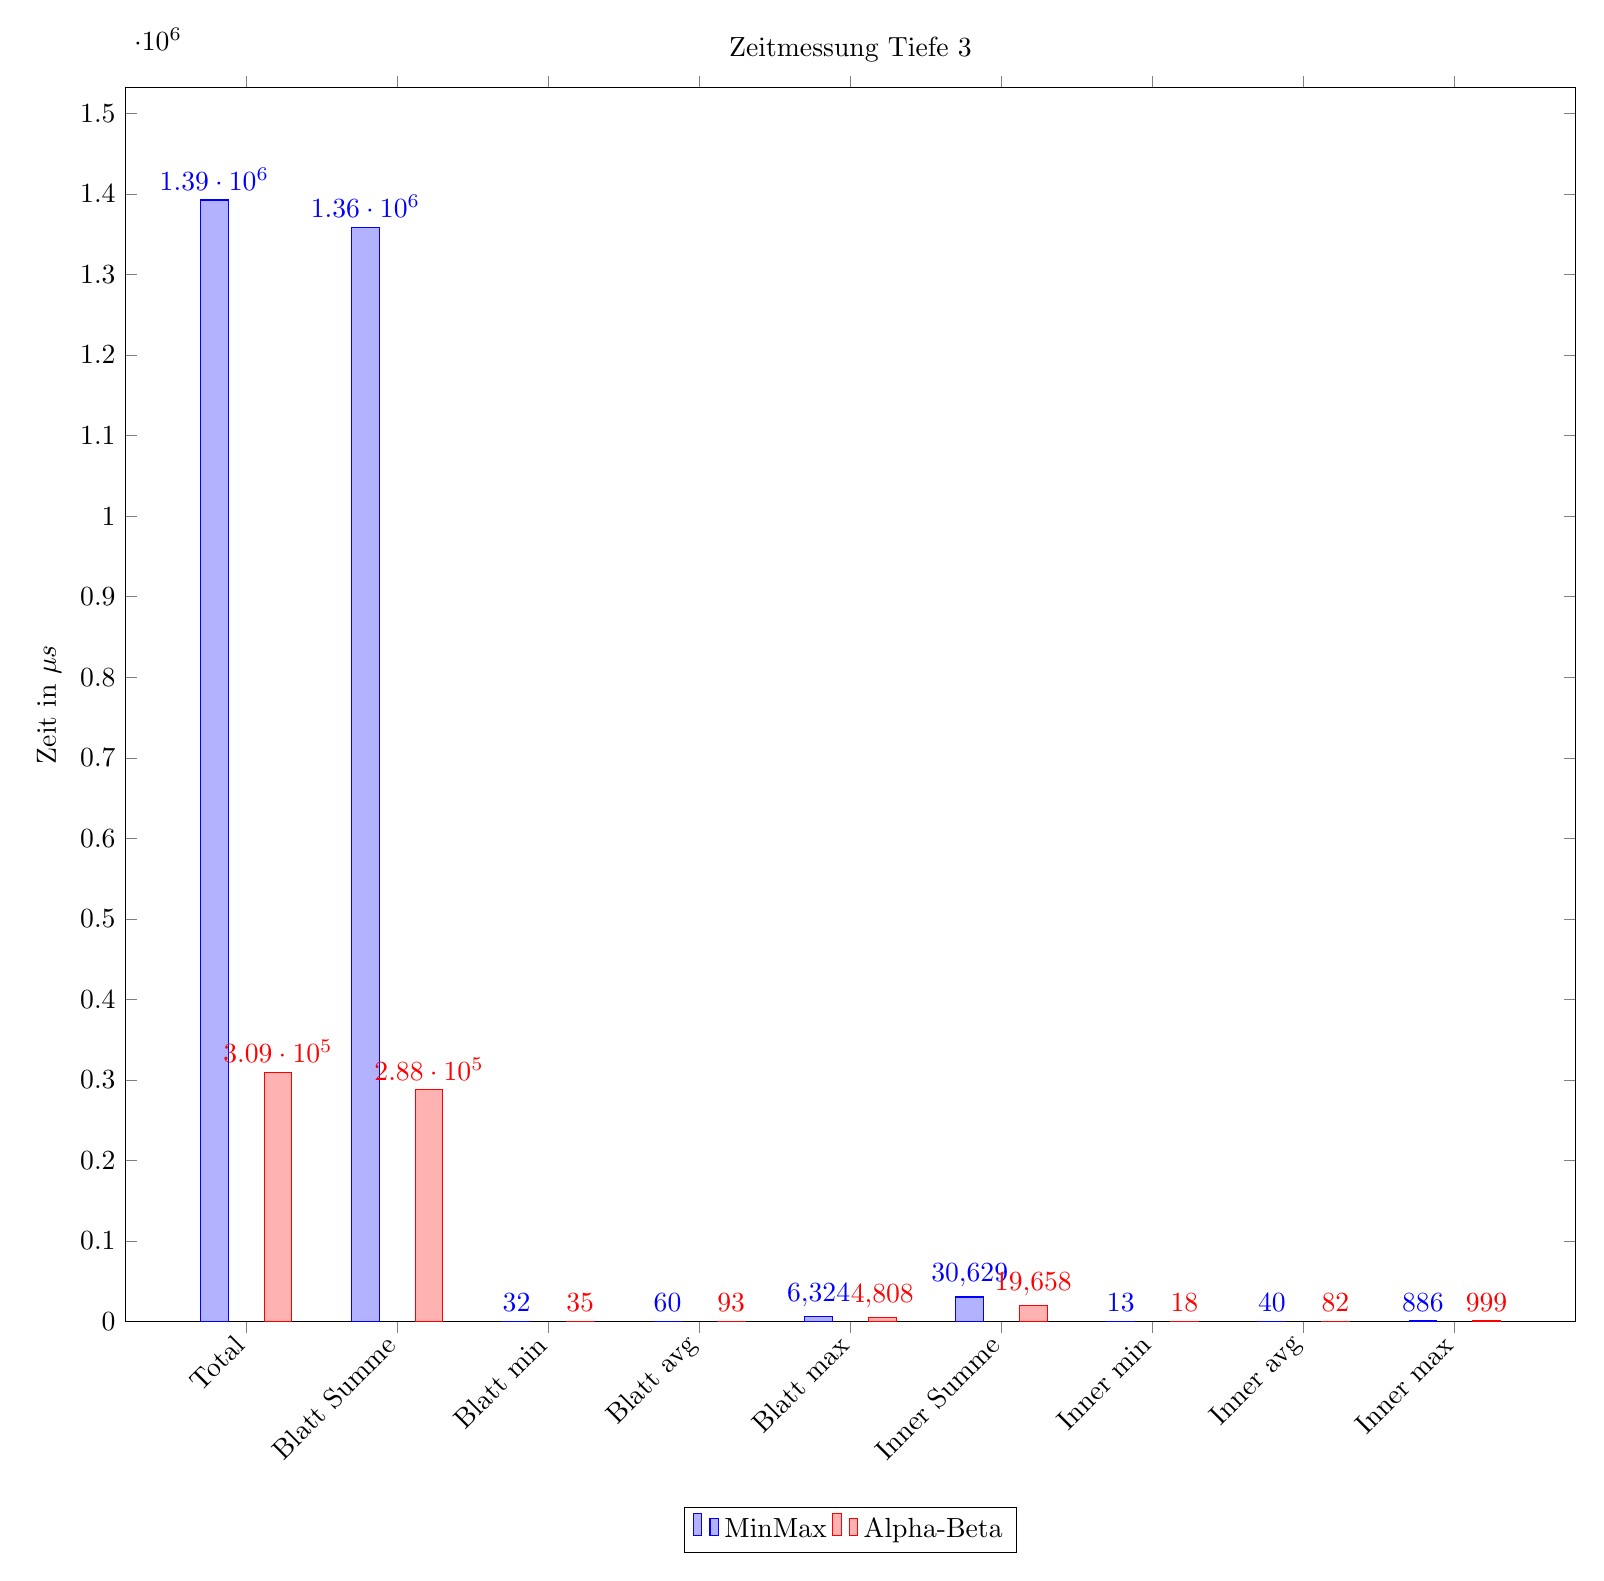
\begin{tikzpicture}
  \begin{axis}[
    title=Zeitmessung Tiefe 3,
    ybar=13pt,
    legend style={at={(0.5,-0.15)},
    anchor=north,
    legend columns=-1},
    ylabel={Zeit in $\mu s$},
    ymin = 0,
    symbolic x coords={
      Total,
      Blatt Summe,
      Blatt min,
      Blatt avg,
      Blatt max,
      Inner Summe,
      Inner min,
      Inner avg,
      Inner max
    },
    xtick=data,
    nodes near coords,
    nodes near coords align={vertical},
    x tick label style={rotate=45,anchor=east}
  ]
    \addplot coordinates{
      (Total,       1392458)
      (Blatt Summe, 1358383)
      (Blatt min,        32)
      (Blatt avg,        60)
      (Blatt max,      6324)
      (Inner Summe,   30629)
      (Inner min,        13)
      (Inner avg,        40)
      (Inner max,       886)
    };
    \addplot coordinates{
      (Total,       309058)
      (Blatt Summe, 287640)
      (Blatt min,       35)
      (Blatt avg,       93)
      (Blatt max,     4808)
      (Inner Summe,  19658)
      (Inner min,       18)
      (Inner avg,       82)
      (Inner max,      999)
    };
    \legend{
      MinMax,
      Alpha-Beta
    }
  \end{axis}
\end{tikzpicture}


\end{document}